\documentclass[a4paper, 12pt]{article}
\usepackage{fontspec}
\usepackage{graphicx}
\usepackage{float}
\usepackage{hyperref}
\usepackage[margin=2cm]{geometry}
\usepackage{amsmath}
\usepackage[polish]{babel}
\usepackage[nottoc,numbib]{tocbibind}

\title{\textbf{Symulacja ruchu ludzi w centrum handlowym}}
\author{Paweł Kłeczek \\ \emph{pkleczek@student.agh.edu.pl} \and Kajetan Rzepecki \\ \emph{kajetan.rzepecki+agh@gmail.com}}
\date{\today}

\begin{document}

    \maketitle

    \vfill
    \begin{abstract}
    % TODO Trzeba dodać coś więcej IMO, na przykład o tym, jak podejdziemy do problemu ruchu ludzi.

\noindent
Praca i związany z nią projekt dotyczą symulowania ruchu ludzi w centrum handlowym z wykorzystaniem modelu \emph{Social Distances} na dwuwymiarowej siatce.
    \end{abstract}
    \vfill

    \thispagestyle{empty} % Nie chcemy numerować pierwszej strony.

\newpage
    \setcounter{page}{1}
    \setcounter{tocdepth}{3}

    \tableofcontents

\newpage
    \section{Wprowadzenie}
    \label{sec:intro}

\noindent
Celem wykonywanego projektu jest stworzenie modelu oraz symulacja ruchu ludzi w centrum handlowym w oparciu m.in. o model \emph{Social Distances} (\cite{refs:social-distances-1, refs:social-distances-2}).

Modelowanie ruchu dużych grup ludzi w środowisku zorganizowanym jest problemem złożonym i wymaga wykorzystania równie złożonych algorytmów celem dokładnego przybliżenia rzeczywistych zachowań. Dobrym podejściem jest dekompozycja problemu modelowania złożonego zjawiska na mniejsze, łatwiejsze do rozwiązania podproblemy, którymi zajmują się osobne, dobrze zdefiniowane i wyspecjalizowane algorytmy i ponowne połączenie wyników ich działania w spójną całość - metoda \emph{Divide and Conquer}.

    \begin{figure}[H]
        \centering
        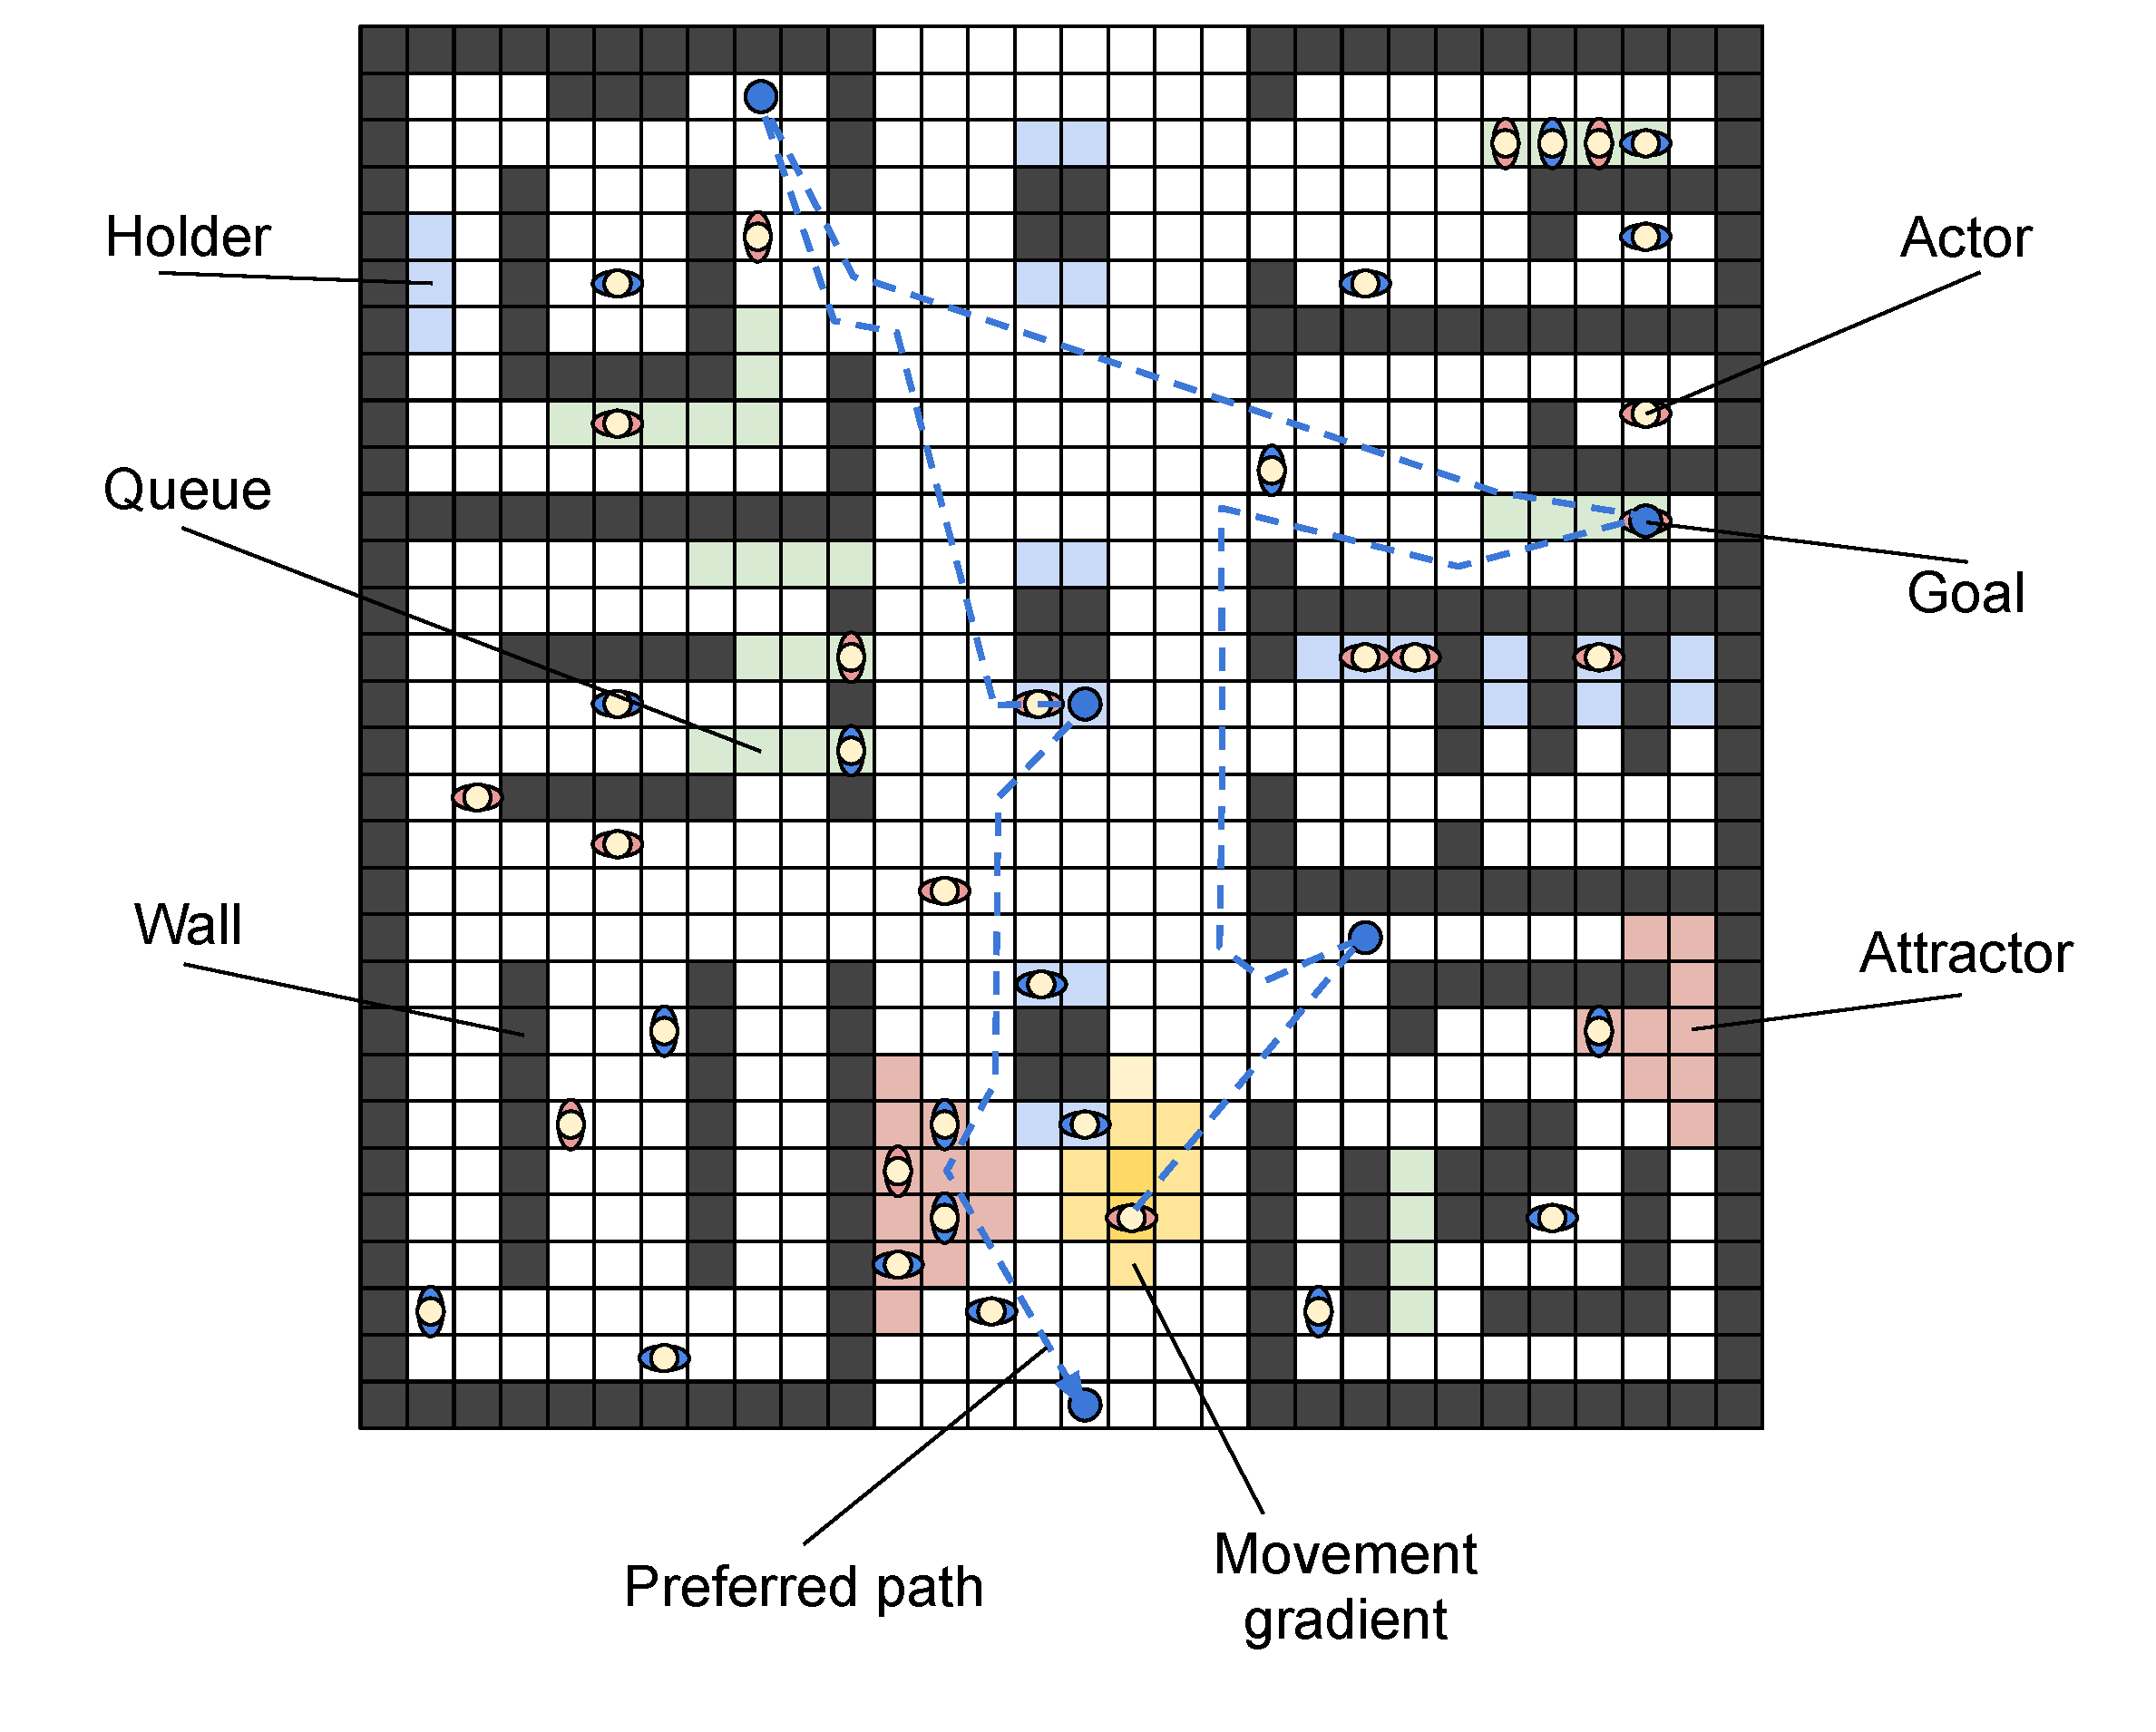
\includegraphics[scale=0.3]{./img/Overview.pdf}
        \caption{Przykładowa dekompozycja problemu modelowania ruchu ludzi w centrum handlowym.}
        \label{fig:decomp}
    \end{figure}

W zależności od domeny rozwiązywanego problemu dekompozycja może zachodzić ze względu na wiele czynników i dotyczyć różnych aspektów problemu - np. podział wejściowego zbioru danych na dwa mniejsze podzbiory w algorytmie \emph{Quick sort}, czy podział modelu ruchu ludzi na elementarne zachowania, jak \emph{kolejkowanie}, \emph{atrakcja} lub \emph{oczekiwanie}.

Na rysunku \ref{fig:decomp} została przedstawiona przykładowa dekompozycja problemu poruszanego w tym dokumencie. Wyszczególniono w niej podział na globalną, preferowaną ścieżkę wiodącą poruszającego się po centrum handlowym agenta do obranych przez niego celów i lokalny ruch zgodny z gradientem ruchu obliczonym na podstawie jego otoczenia. Dodatkowo zastosowano podział na specjalne strefy odpowiedzialne za modelowanie elementarnych zachowań ludzi w centrach handlowych, takie jak strefy kolejek, czekania i gromadzenia się, które realizowane są za pomocą innych modeli ruchu.

\newpage
    \subsection{State of the art}
    \label{sec:sota}

\noindent
Zagadnienia modelowania ruchu ludzi są od długiego czasu postrzegane jako istotne z punktu widzenia usługowego. Już w latach 80 ubiegłego wieku Aloys Borgers i Harry Timmermans zajmowali się modelowaniem ruchu pieszych w środowisku centrum handlowego  (\cite{refs:route-choice-1}).
Na przestrzeni lat modele te ewoluowały w wielu kierunkach, od automatów komórkowych (\cite{refs:cellural-movement}) przez systemy agentowe (\cite{refs:real-data-2}) aż do modeli probabilistycznych i opartych o algorytmy genetyczne (\cite{refs:pedestrian-behaviour-2}). \\

% TODO Opisać refs:cellural-movement
% TODO Opisać refs:pedestrian-behaviour-2
% TODO Opisać refs:real-data-2

Więcej interesujących publikacji związanych z tematyką tego projektu zawarto w secji \ref{sec:refs}.

\newpage
    \section{Model centrum handlowego}
    \label{sec:mall-model}

\noindent
Zgodnie z metodą \emph{Divide and Conquer} zaproponowaną we \hyperref[sec:intro]{wprowadzeniu}, zdecydowano się na dekompozycję problemu modelowania ruchu ludzi w centrum handlowym na elementarne, abstrakcyjne zachowania oraz, ze względu na cele poszczególnych agentów i sposoby ich osiągania, na globalne i lokalne planowanie trasy podróży, co zawarto na rysunku \ref{fig:overview}.

    \begin{figure}[H]
        \centering
        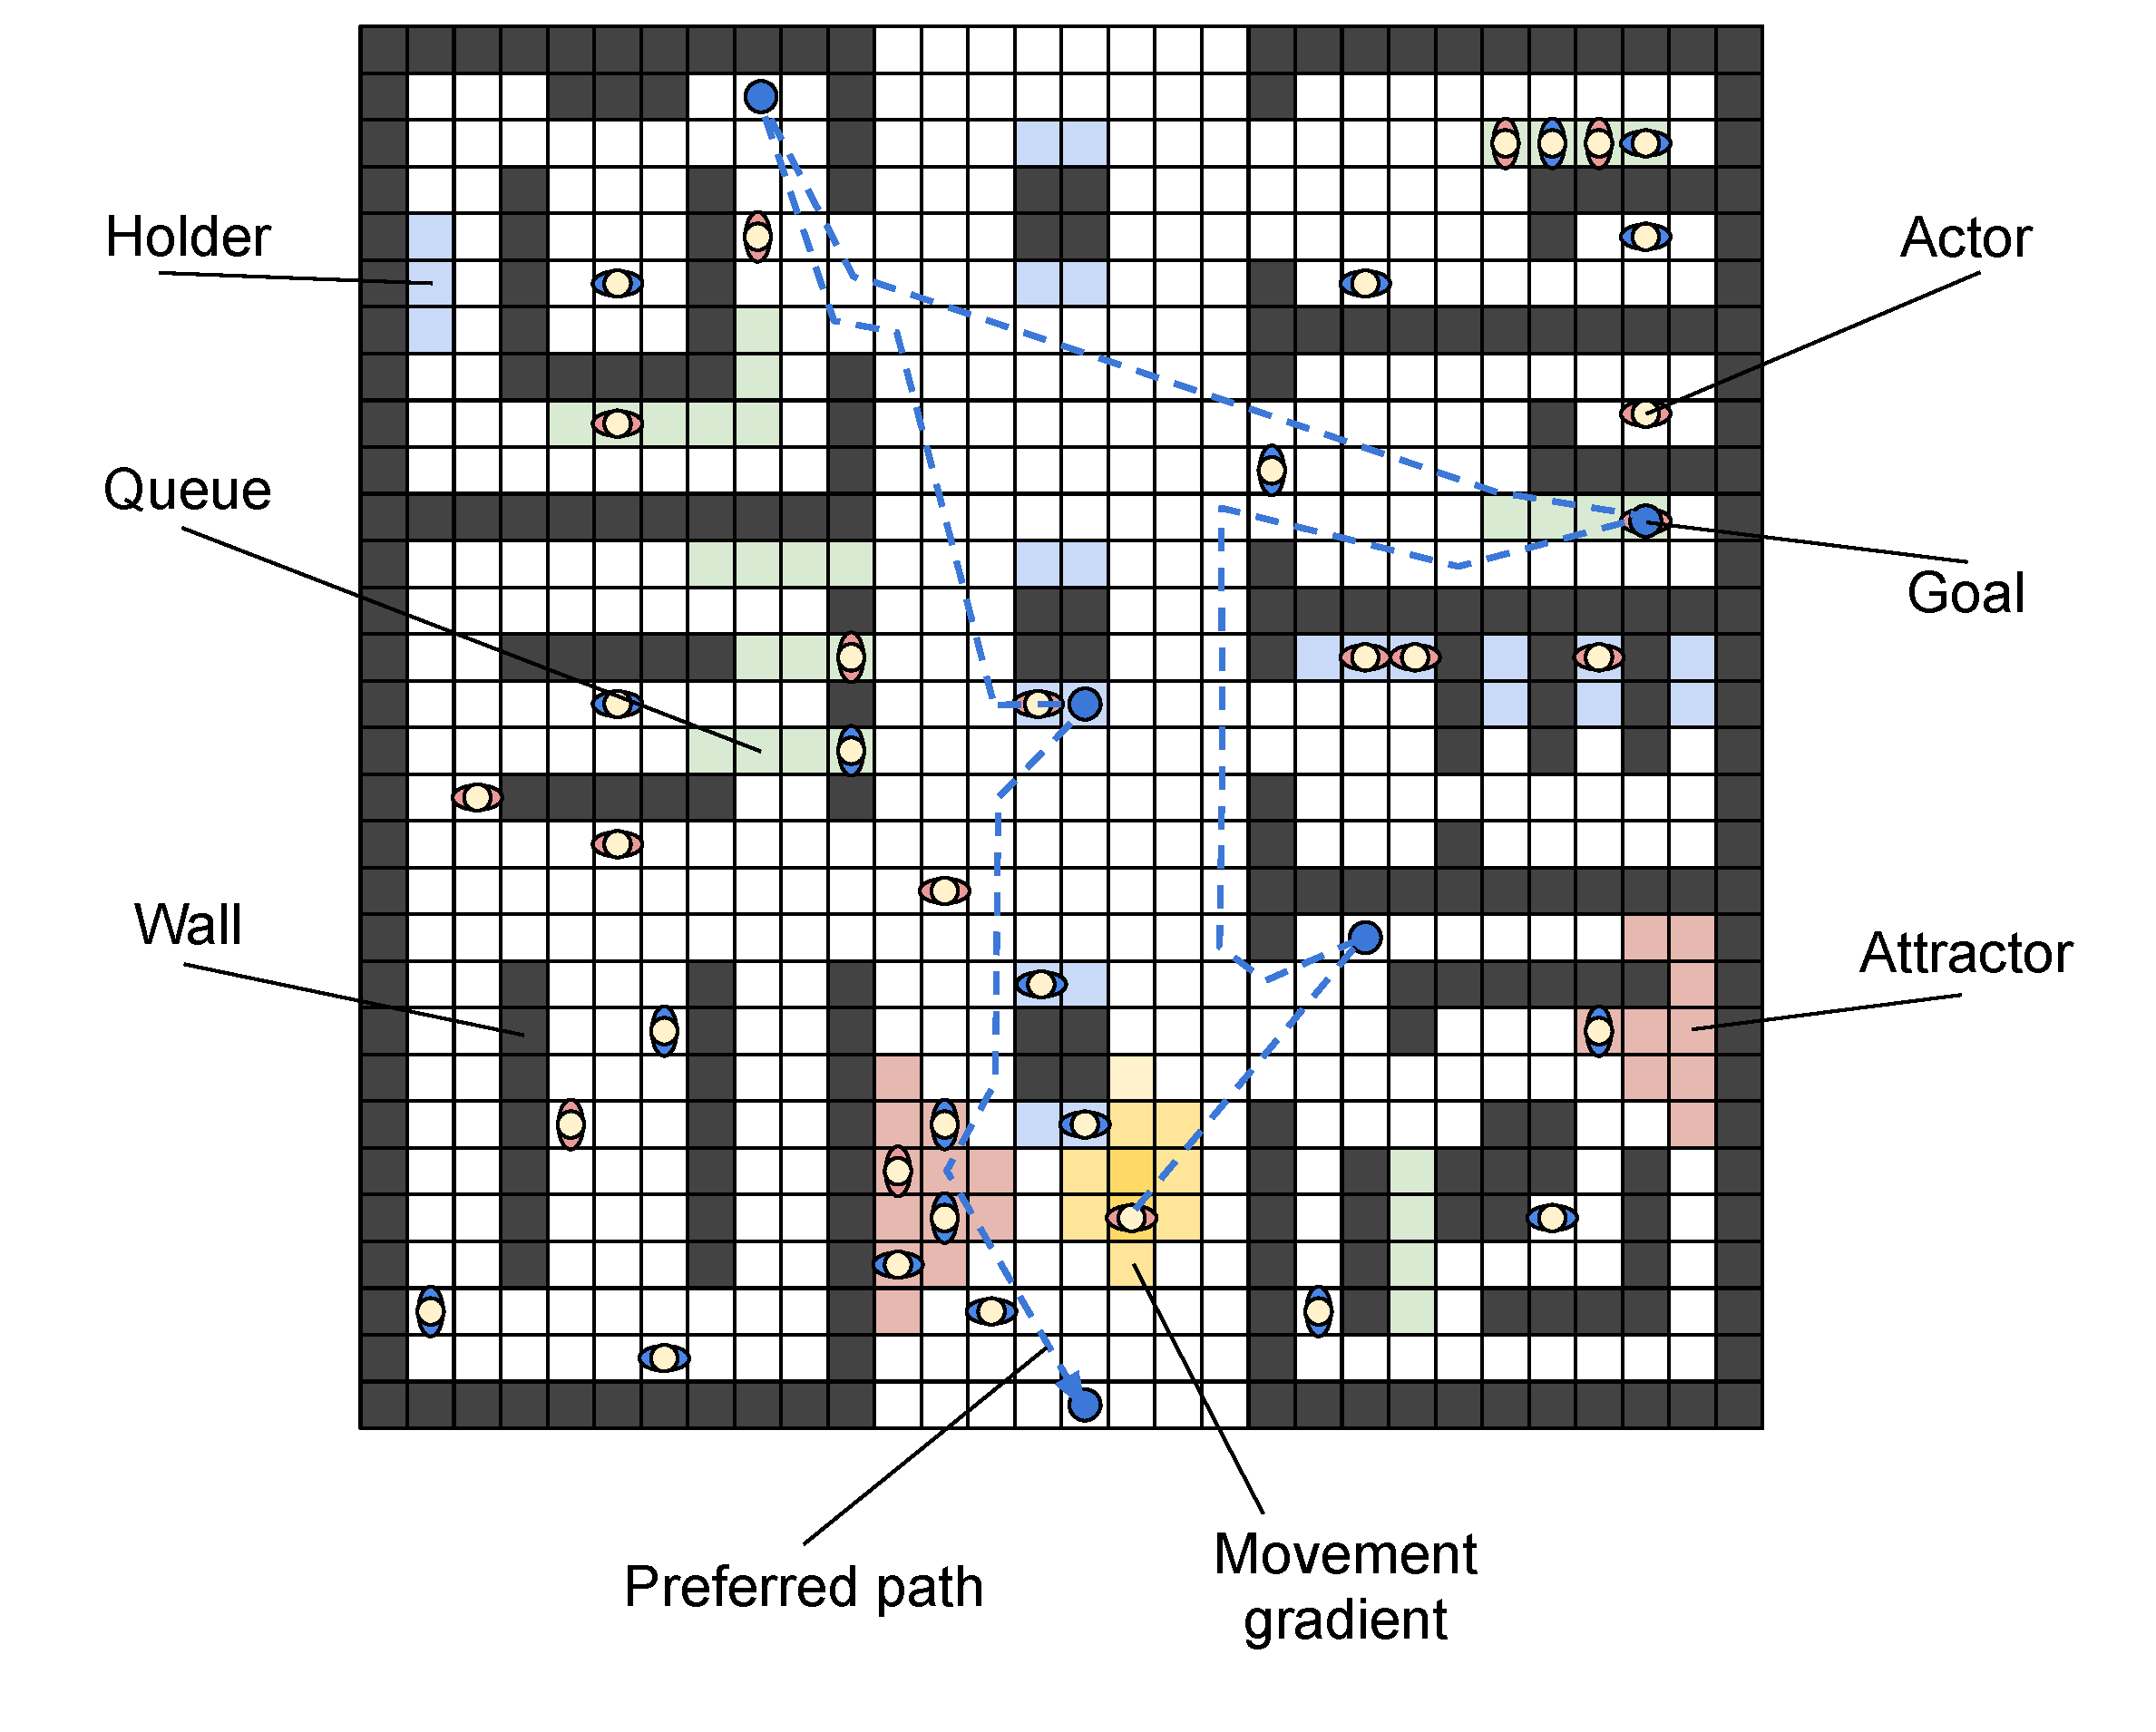
\includegraphics[scale=0.3]{./img/Overview.pdf}
        \caption{Zastosowana dekompozycja problemu.}
        \label{fig:overview}
    \end{figure}

Model centrum handlowego przewiduje istnienie specjalnych stref, wewnątrz których algorytmy odpowiedzialne za poruszanie agentów są modyfikowane lub zastępowane celem modelowania dobrze zdefiniowanych elementarnych zachowań, takich jak \emph{kolejkowanie}, czy \emph{grupowanie się}. W wyniku obserwacji stwierdzono istnienie czterech rodzajów stref specjalnych - strefy przyciągania uwagi (atraktory), kolejki, przejścia i miejsca przeznaczone do czekania. 

    \subsection{Atraktory}
    \label{sec:attractors}

Atraktor jest specjalną strefą charakteryzującą się podwyższonym zainteresowaniem ze strony agentów poruszających się po centrum handlowym. Atraktor ma za zadanie modelować obecność przedmiotu lub zjawiska, które przykuwa uwagę ludzi na terenie centrum handlowego, a wynikiem jego działania jest spontaniczne powstawanie skupisk ludzi - \emph{grupowanie się}.

    \begin{figure}[H]
        \centering
        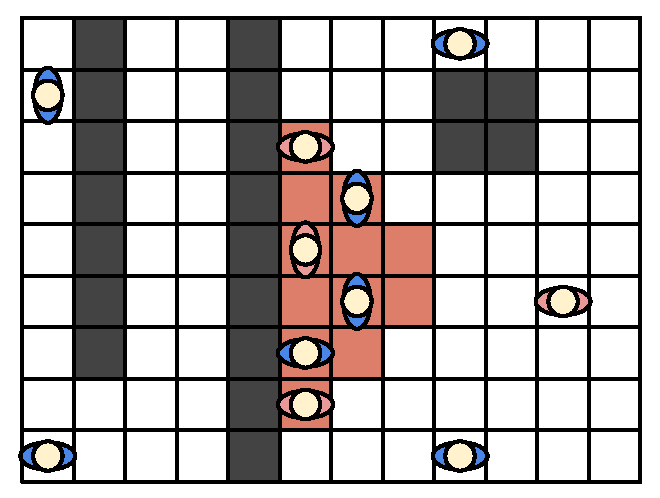
\includegraphics[scale=0.4]{./img/Crowding.pdf}
        \caption{Grupowanie się agentów w obrębie atraktora.}
        \label{fig:crowding}
    \end{figure}

Atraktory różnią się między sobą typami - atraktory różnych typów przyciągają inne rodzaje agentów, co modeluje różnice w preferencjach ludzi przebywających w centrum handlowym. Działanie atraktorów jest najistotniejsze w \hyperref[sec:tactical]{taktycznej} fazie modelu ruchu, w której ma miejsce wybór i modyfikacja preferowanych przez agentów dróg prowadzących do wybranych celów.

    \subsection{Kolejki}
    \label{sec:queues}

Drugim istotnym z punktu widzenia modelu centrum handlowego typem strefy specjalnej jest strefa kolejki. Zadaniem kolejki jest modelowanie zjawiska \emph{ścisłego kolejkowania się} ludzi, na przykład przy kasie sklepowej, lub na stopniach eskalatora, co nie wynika z ogólnego modelu ruchu.

    \begin{figure}[H]
        \centering
        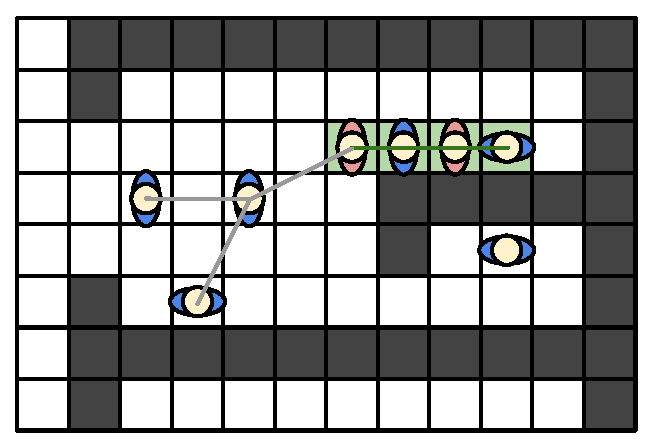
\includegraphics[scale=0.4]{./img/Queueing.pdf}
        \caption{Kolejkowanie się ludzi przy kasie sklepowej z zaznaczoną kolejką ścisłą.}
        \label{fig:queueing}
    \end{figure}

Kolejki modyfikują działanie \hyperref[sec:operational]{fazy operacyjnej} modelu ruchu zmniejszając udział modelu \hyperref[sec:social-dist]{preferencji odległościowych} w wyznaczaniu oceny sąsiadujących z agentem komórek mapy centrum handlowego.

    \subsection{Przejścia/wejścia/wyjścia}
    \label{sec:entrance-exits}

Strefy przejść pozwalają na \emph{tworzenie}, \emph{przemieszczanie} pomiędzy różnymi fragmentami mapy centrum handlowego i \emph{usuwanie} agentów, którzy osiągnęli wszystkie cele swojej podróży.

    \begin{figure}[H]
        \centering
        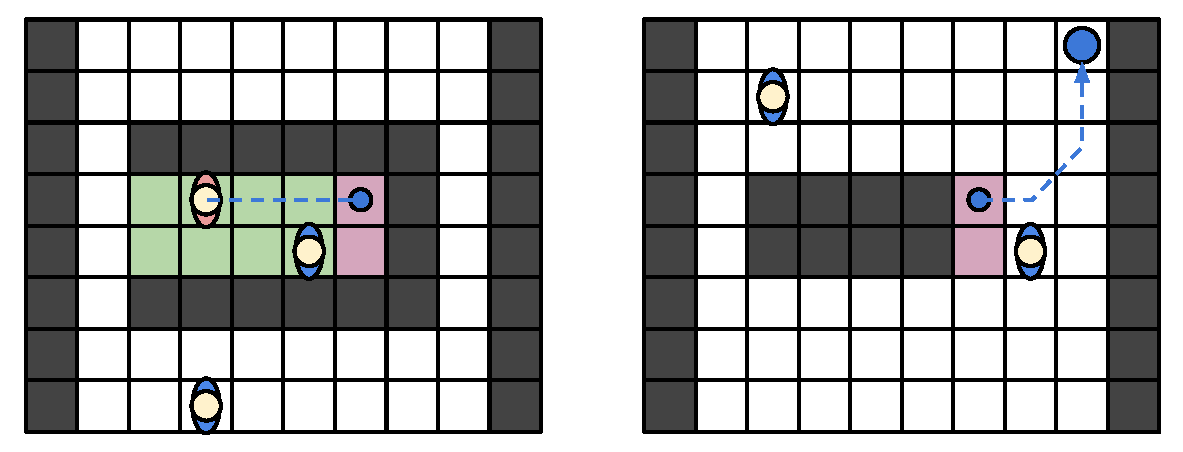
\includegraphics[scale=0.4]{./img/EntranceExits.pdf}
        \caption{Poruszanie się agenta po eskalatorze pomiędzy piętrami centrum handlowego.}
        \label{fig:passing-through}
    \end{figure}

    \subsection{Miejsca oczekiwania}
    \label{sec:holders}

Ostatnim istotnym typem strefy specjalnej jest miejsce oczekiwania, modelujące wszelkiego rodzaju miejsca spędzania czasu w bezruchu. Agent trafiający do miejsca oczekiwania zostaje wstrzymany na ustaloną ilość czasu przed kontynuowaniem swojej podróży.

    \begin{figure}[H]
        \centering
        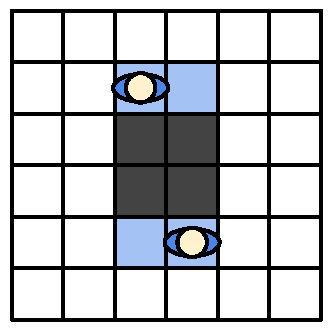
\includegraphics[scale=0.4]{./img/Held.pdf}
        \caption{Agenci oczekujący końca świata.}
        \label{fig:held-down}
    \end{figure}

\newpage
    \section{Model ruchu ludzi}
    \label{sec:move-model}

\noindent
W zastosowanym algorytmie można wyszczególnieć dwie główne, wzajemnie od siebie zależne fazy - fazę \hyperref[sec:tactical]{taktyczną} oraz fazę \hyperref[sec:operational]{operacyjną}, których interakcję przestawiono na poniższym, uproszczonym diagramie.

    \begin{figure}[H]
        \centering
        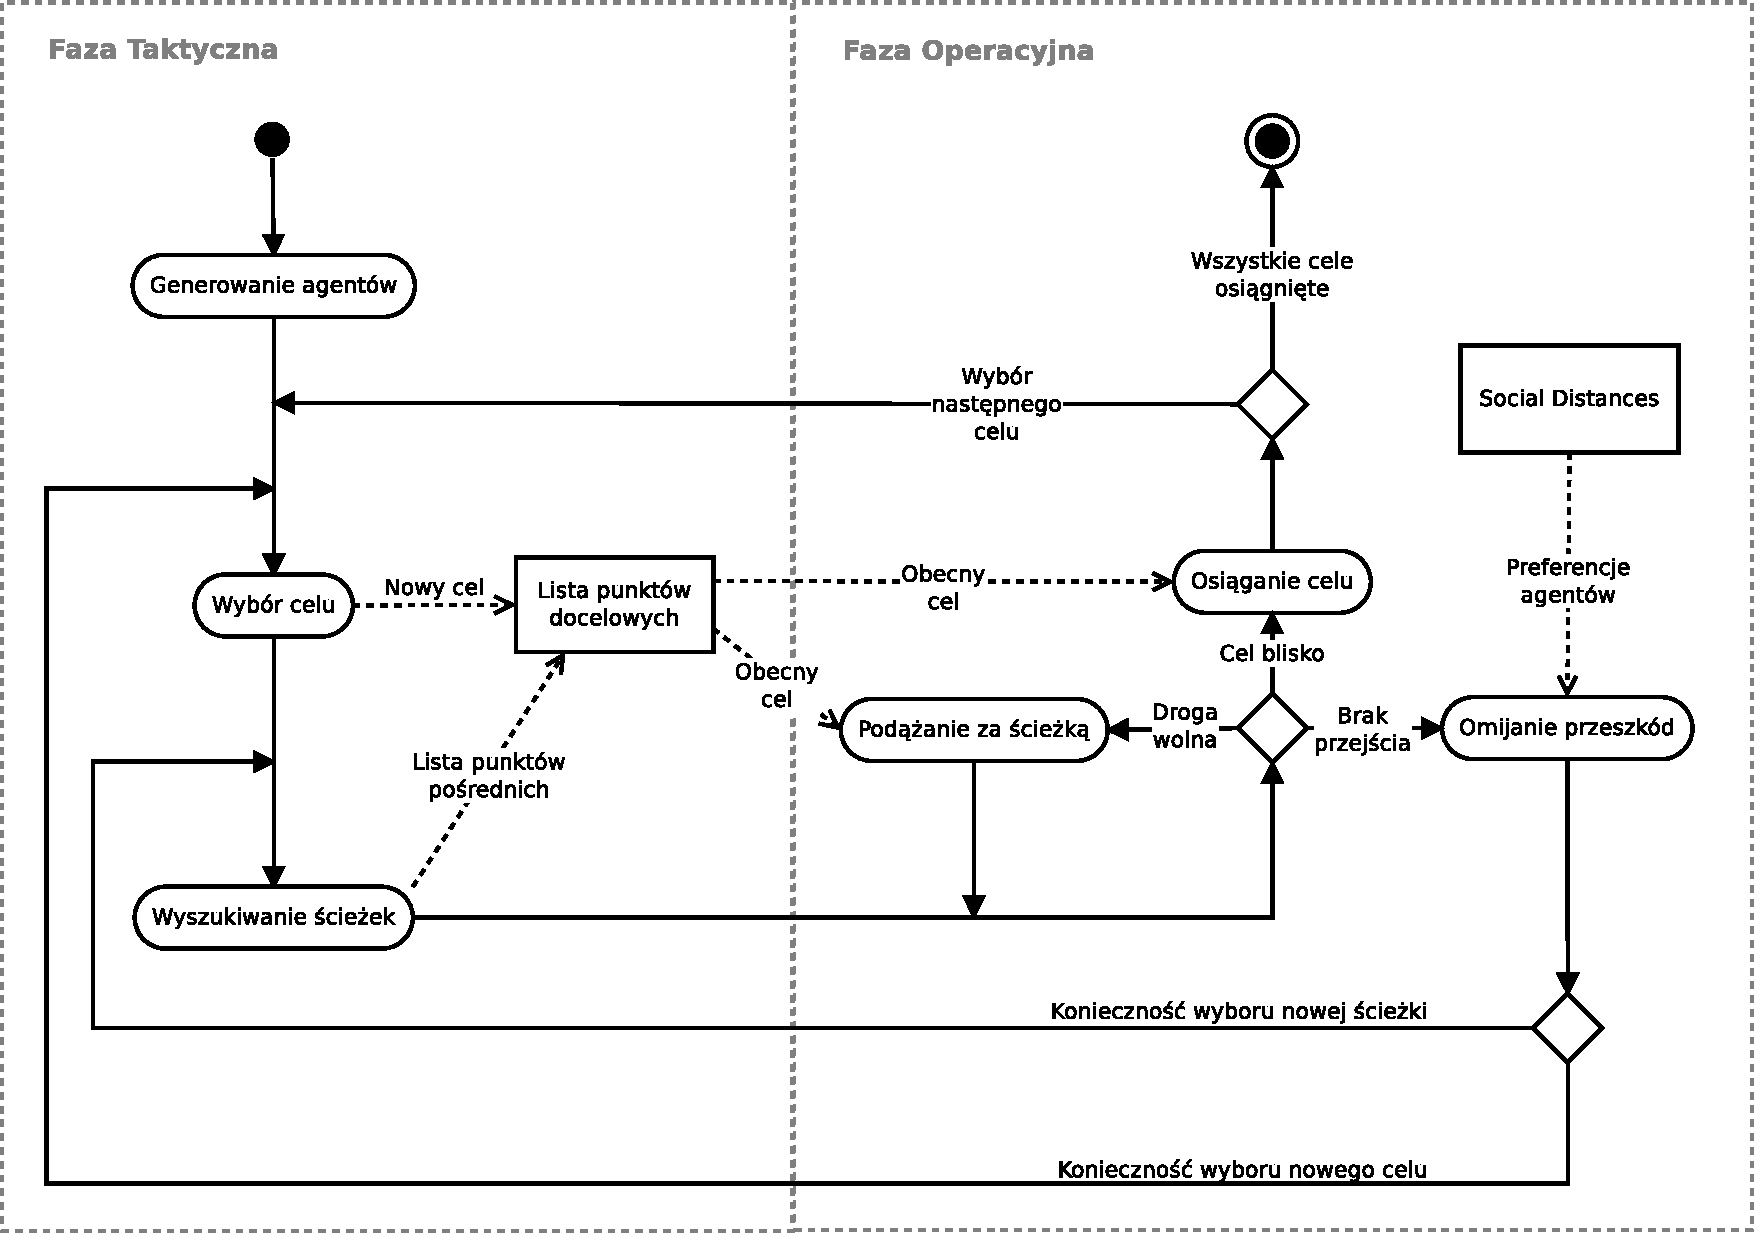
\includegraphics[scale=0.7]{./img/ActorActivity.pdf}
        \caption{Diagram aktywności agentów.}
        \label{fig:actor-activity}
    \end{figure}

    % TODO Więcej szczegółów na temat generowania aktora i zestawu jego parametrów.
    % TODO Więcej szczegółów na temat algorytmu wybierania miejsc docelonych.

Algorytm rozpoczyna pracę od wygenerowania agenta na podstawie wcześniej zdefiniowanych archetypów.
Dla każdego agenta wybierana jest wstępna lista miejsc docelowych, które zostaną przez niego odwiedzone w czasie działania symulacji, oraz obliczana jest optymalna ścieżka wiodące do pierwszego wybranego w poprzednim kroku miejsca docelowego. Algorytm następnie modyfikuje ścieżkę w oparciu o mapę rozkładu stref specjalnych centrum handlowego by lepiej modelować faktyczne zamiary danego aktora.

Po wygenerowaniu niezbędnych danych taktycznych dla każdego agenta algorytm przechodzi do fazy operacyjnej, która odpowiada za właściwe przemieszczanie agentów. Faza ta zachodzi w lokalnym otoczeniu każdego agenta i odpowiada za zachowania takie jak omijanie przeszkód, grupowanie się, podążanie za obraną ścieżką i inne akcje związane ze specjalnymi strefami centrum handlowego.
Algorytm na podstawie bezpośredniego otoczenia agenta oraz metadanych dotyczących obecnego celu jego podróży podejmuje decyzje o możliwości wykonania ruchu, lub w przypadku skrajnym o modyfikacji wybranej ścieżki prowadzącej do celu, czy nawet zmianie aktualnego celu podróży.
W przypadku osiągnięcia miejsca docelowego algorytm przechodzi do rozpatrywania następnego miejsca docelowego, lub w tryb ``błądzenia'', gdy osiągnięto już wszystkie wyznaczone cele.

\newpage
        \subsection{Faza taktyczna}
        \label{sec:tactical}

        \begin{figure}[H]
            \centering
            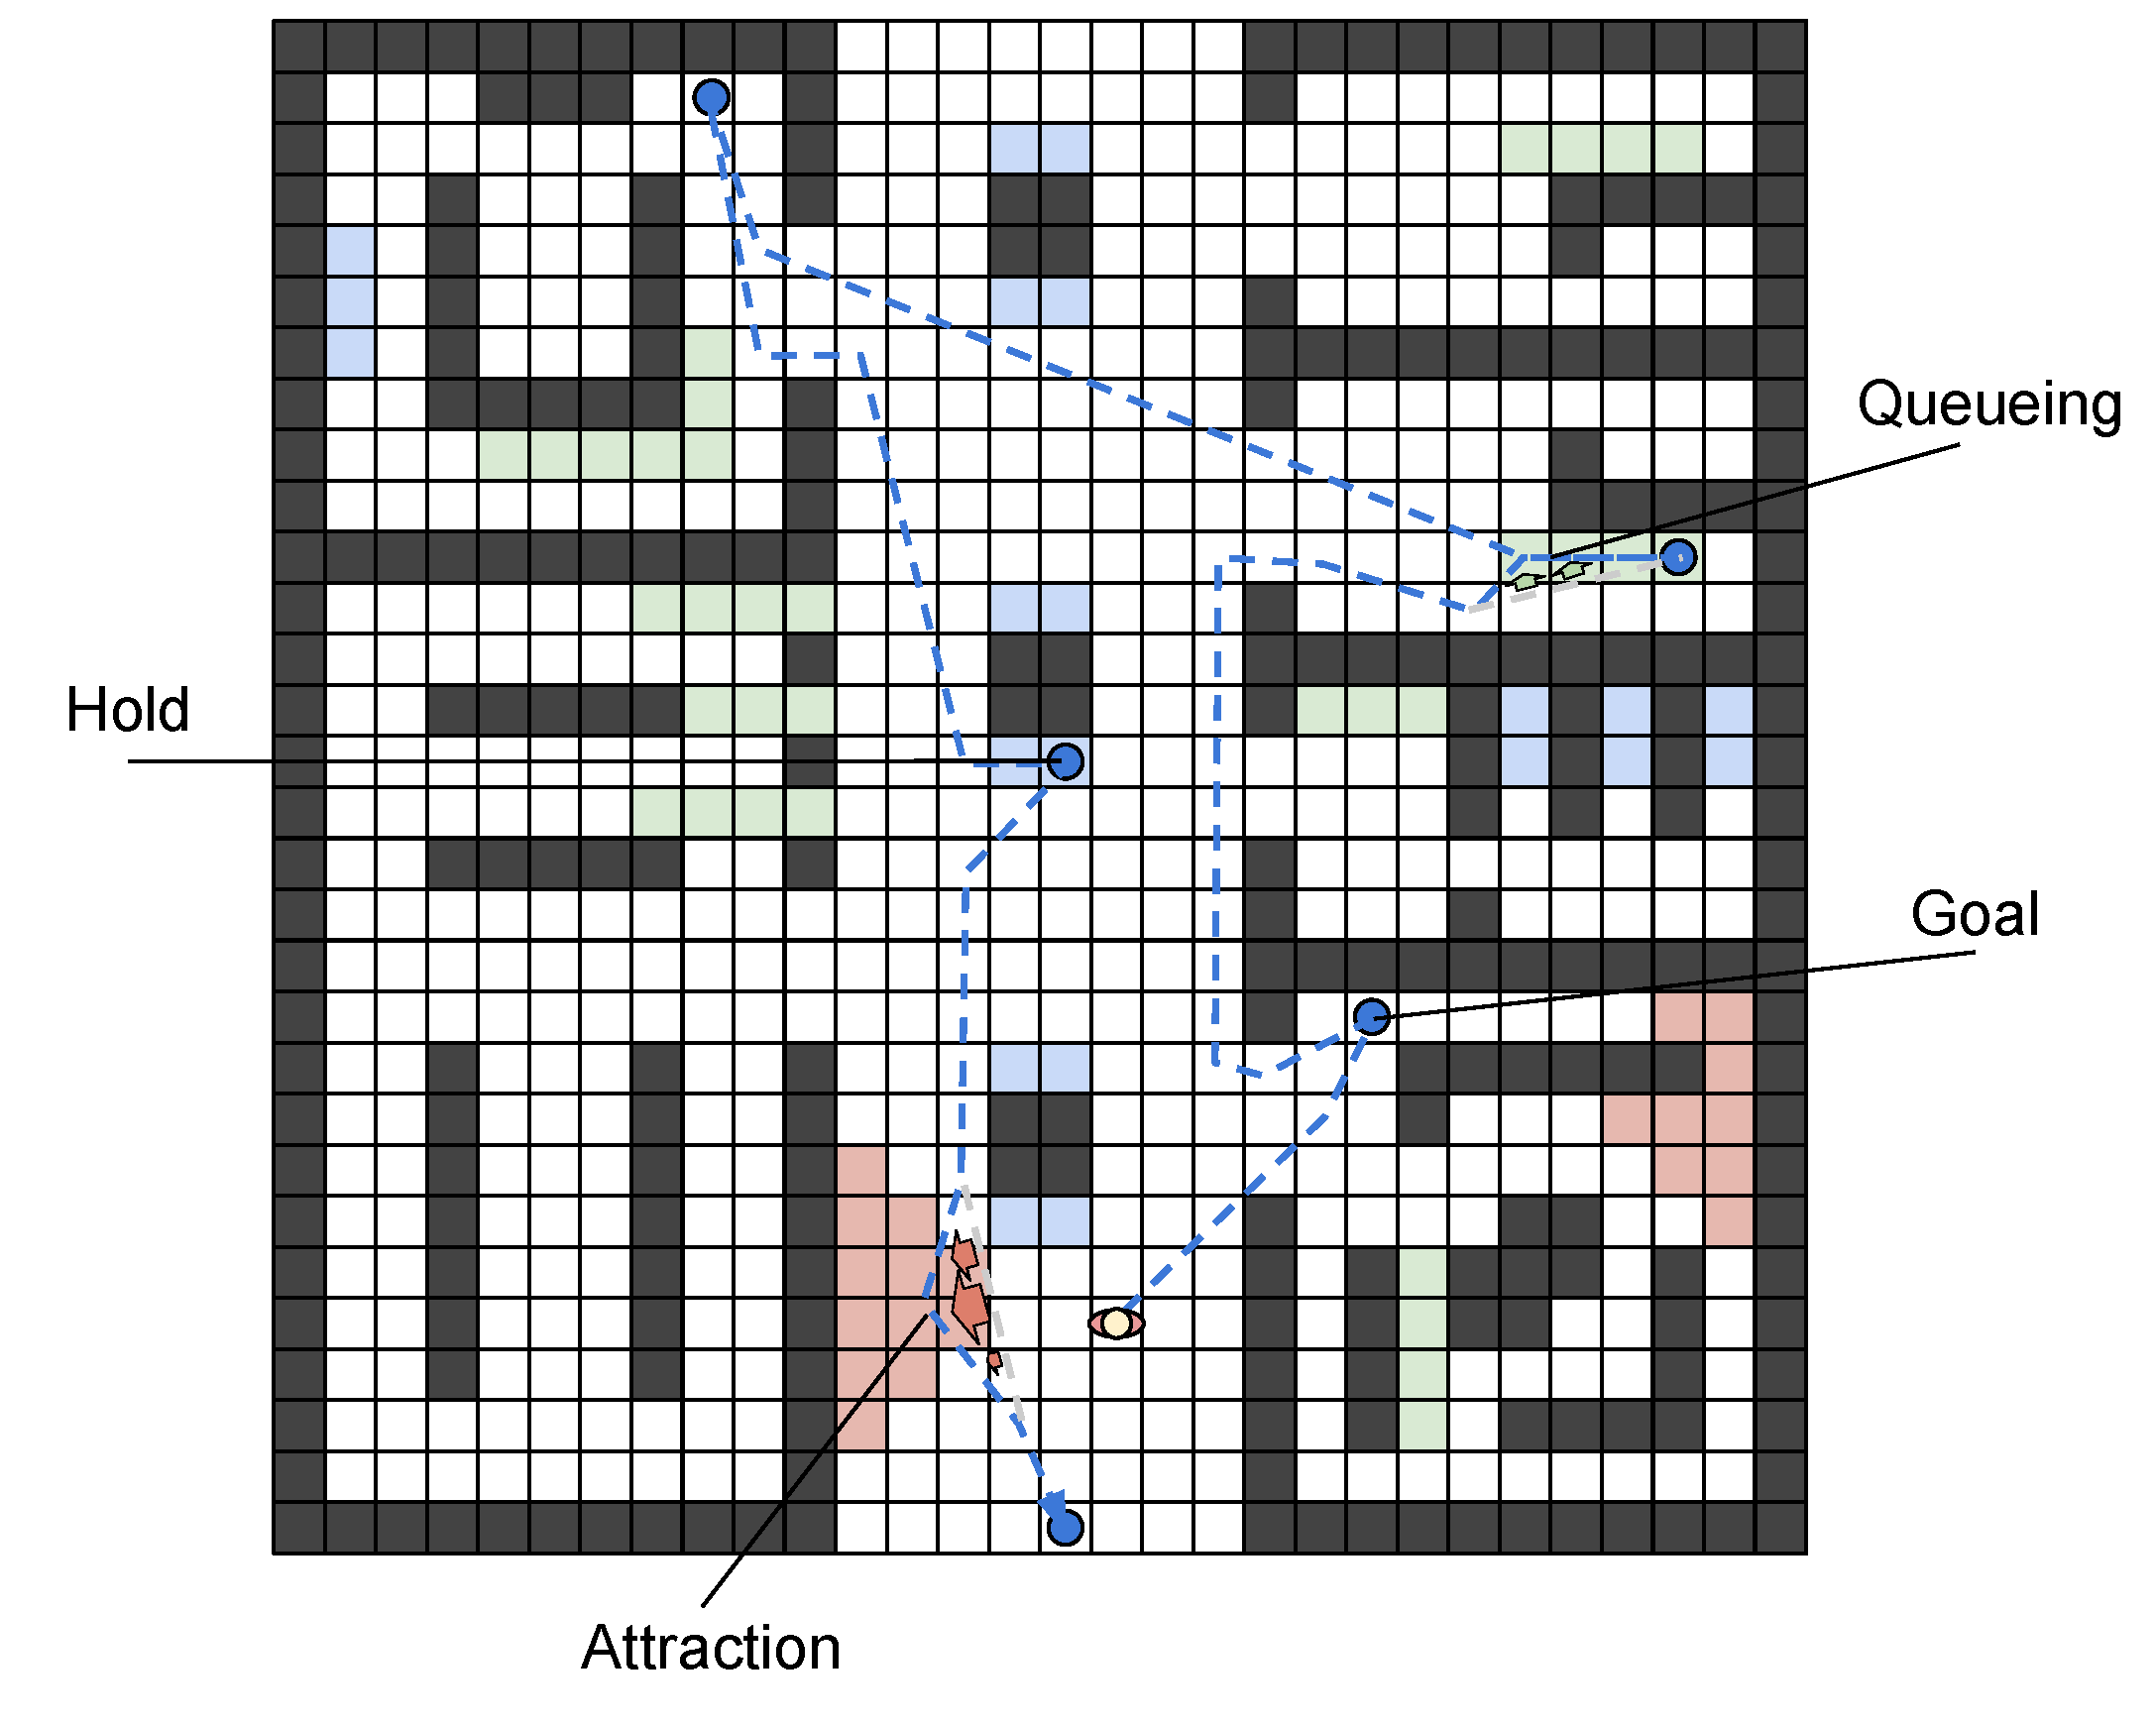
\includegraphics[scale=0.3]{./img/Tactical.pdf}
            \caption{Zakres operacji taktycznej części modelu ruchu.}
            \label{fig:tactical}
        \end{figure}

        % TODO Linki do opisu atraktorów, kolejek itd.

\noindent
Faza taktyczna zachodzi globalnie dla każdego agenta bez uwzględnienia jego lokalnego otoczenia, innych agentów, czy fizycznych właściwości centrum handlowego - nie jest istotnym, czy dany korytarz został zablokowany przez grupę ludzi i nie umożliwia przejścia. Faza ta modeluje abstrakcyjne zamiary agenta i jej celem jest przede wszystkim wybór listy miejsc docelowych oraz wyznaczenie dróg do nich prowadzących, co zostało osiągnięte dzięki \hyperref[sec:path-finding]{algorytmowi znajdowania ścieżek} oraz \hyperref[sec:mall-impl]{mapie rozkładu stref specjalnych} centrum handlowego. Pod uwagę brane są \hyperref[sec:attractors]{atraktory}, \hyperref[sec:queues]{kolejki} i \hyperref[sec:entrance-exits]{przejścia}, które algorytm stara się osiągnąć modyfikując wcześniej wyznaczoną, optymalną ścieżkę prowadzącą do aktualnego celu podróży.

        \subsection{Faza operacyjna}
        \label{sec:operational}

        \begin{figure}[H]
            \centering
            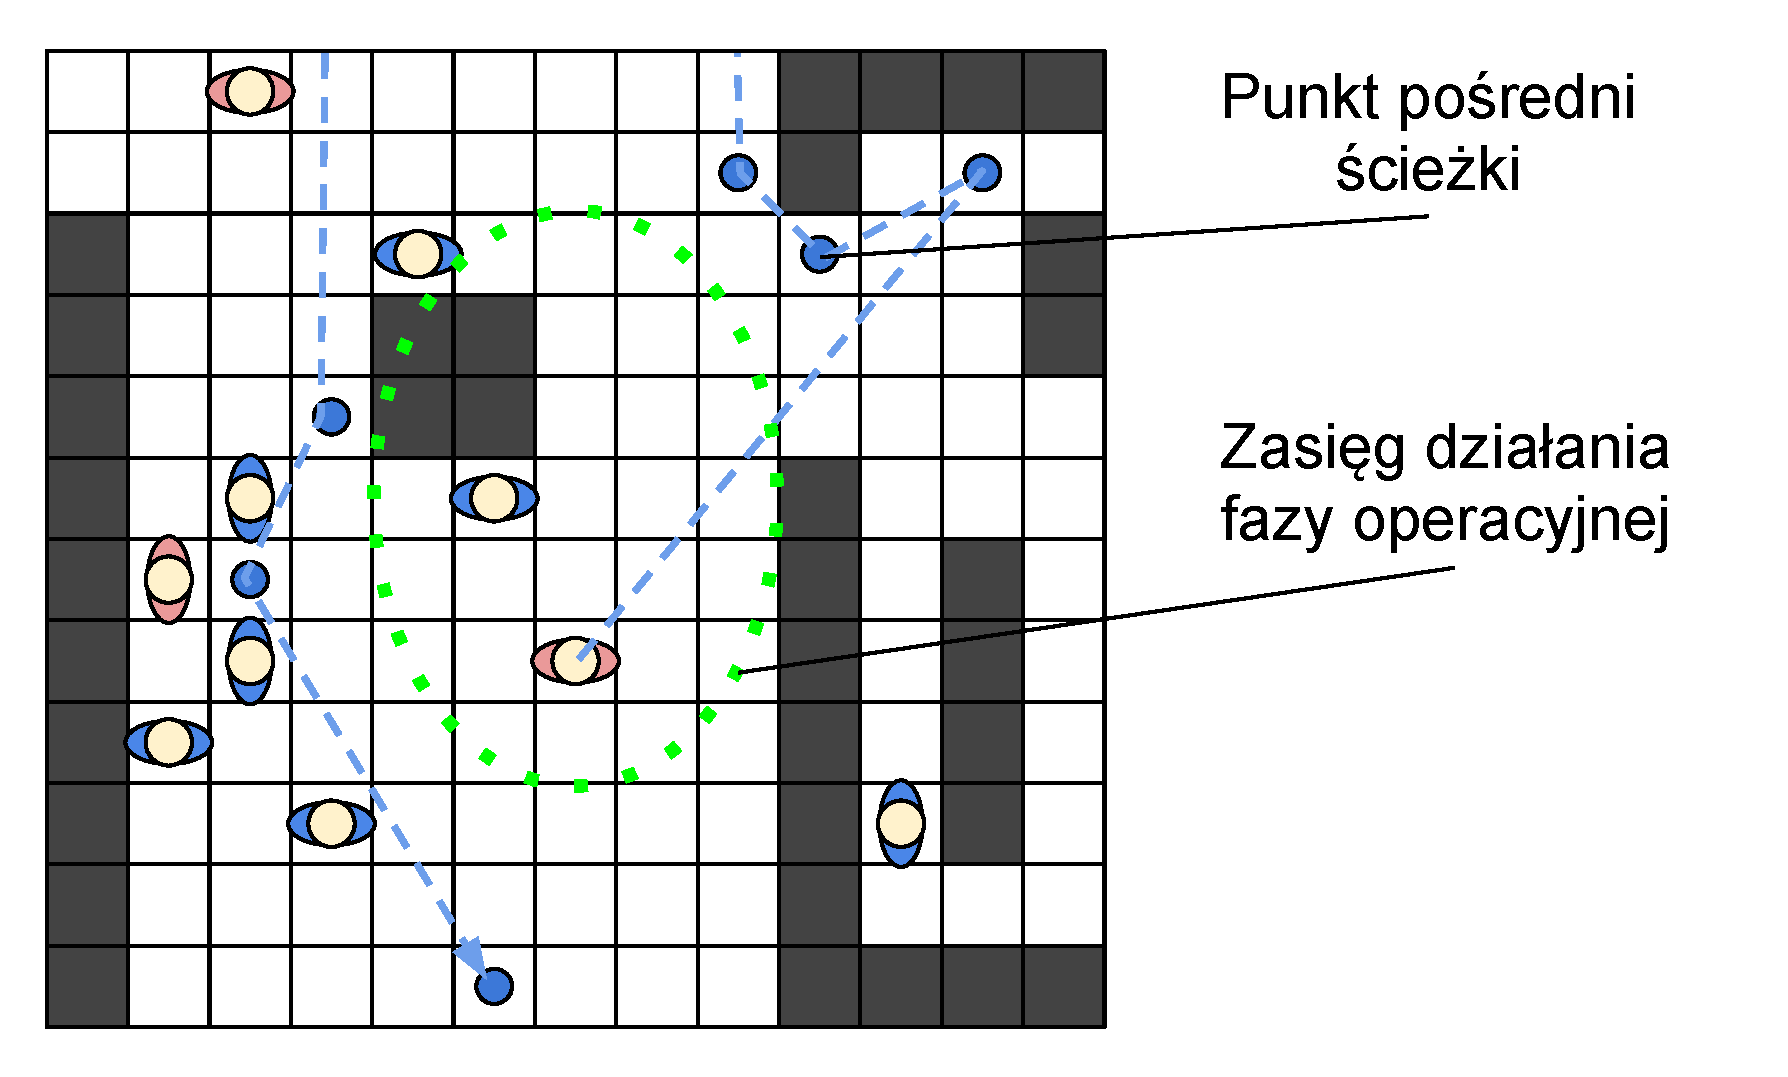
\includegraphics[scale=0.3]{./img/Operative.pdf}
            \caption{Zakres działania operacyjnej części modelu ruchu.}
            \label{fig:operational}
        \end{figure}

        % TODO Potrzeba większego opisu, który bardziej zagłębia się w wybrany algorytm operacyjny.

\noindent
Faza operacyjna zachodzi w lokalnym otoczeniu każdego agenta, a jej celem jest wykonanie właściwego ruchu agenta. Faza ta jest odpowiedzialna za unikanie kolizji i omijanie przeszkód. Pod uwagę brani są inni agenci oraz metadane dotyczące drogi prowadzącej do aktualnego celu podróży wygenerowane w taktyczniej fazie działania algorytmu.

\newpage
    \section{Implementacja}
    \label{sec:implementation}

     % TODO Opisać technikalia implementacji...

        \subsection{Reprezentacja centrum handlowego}
        \label{sec:mall-impl}

        \begin{figure}[H]
            \centering
            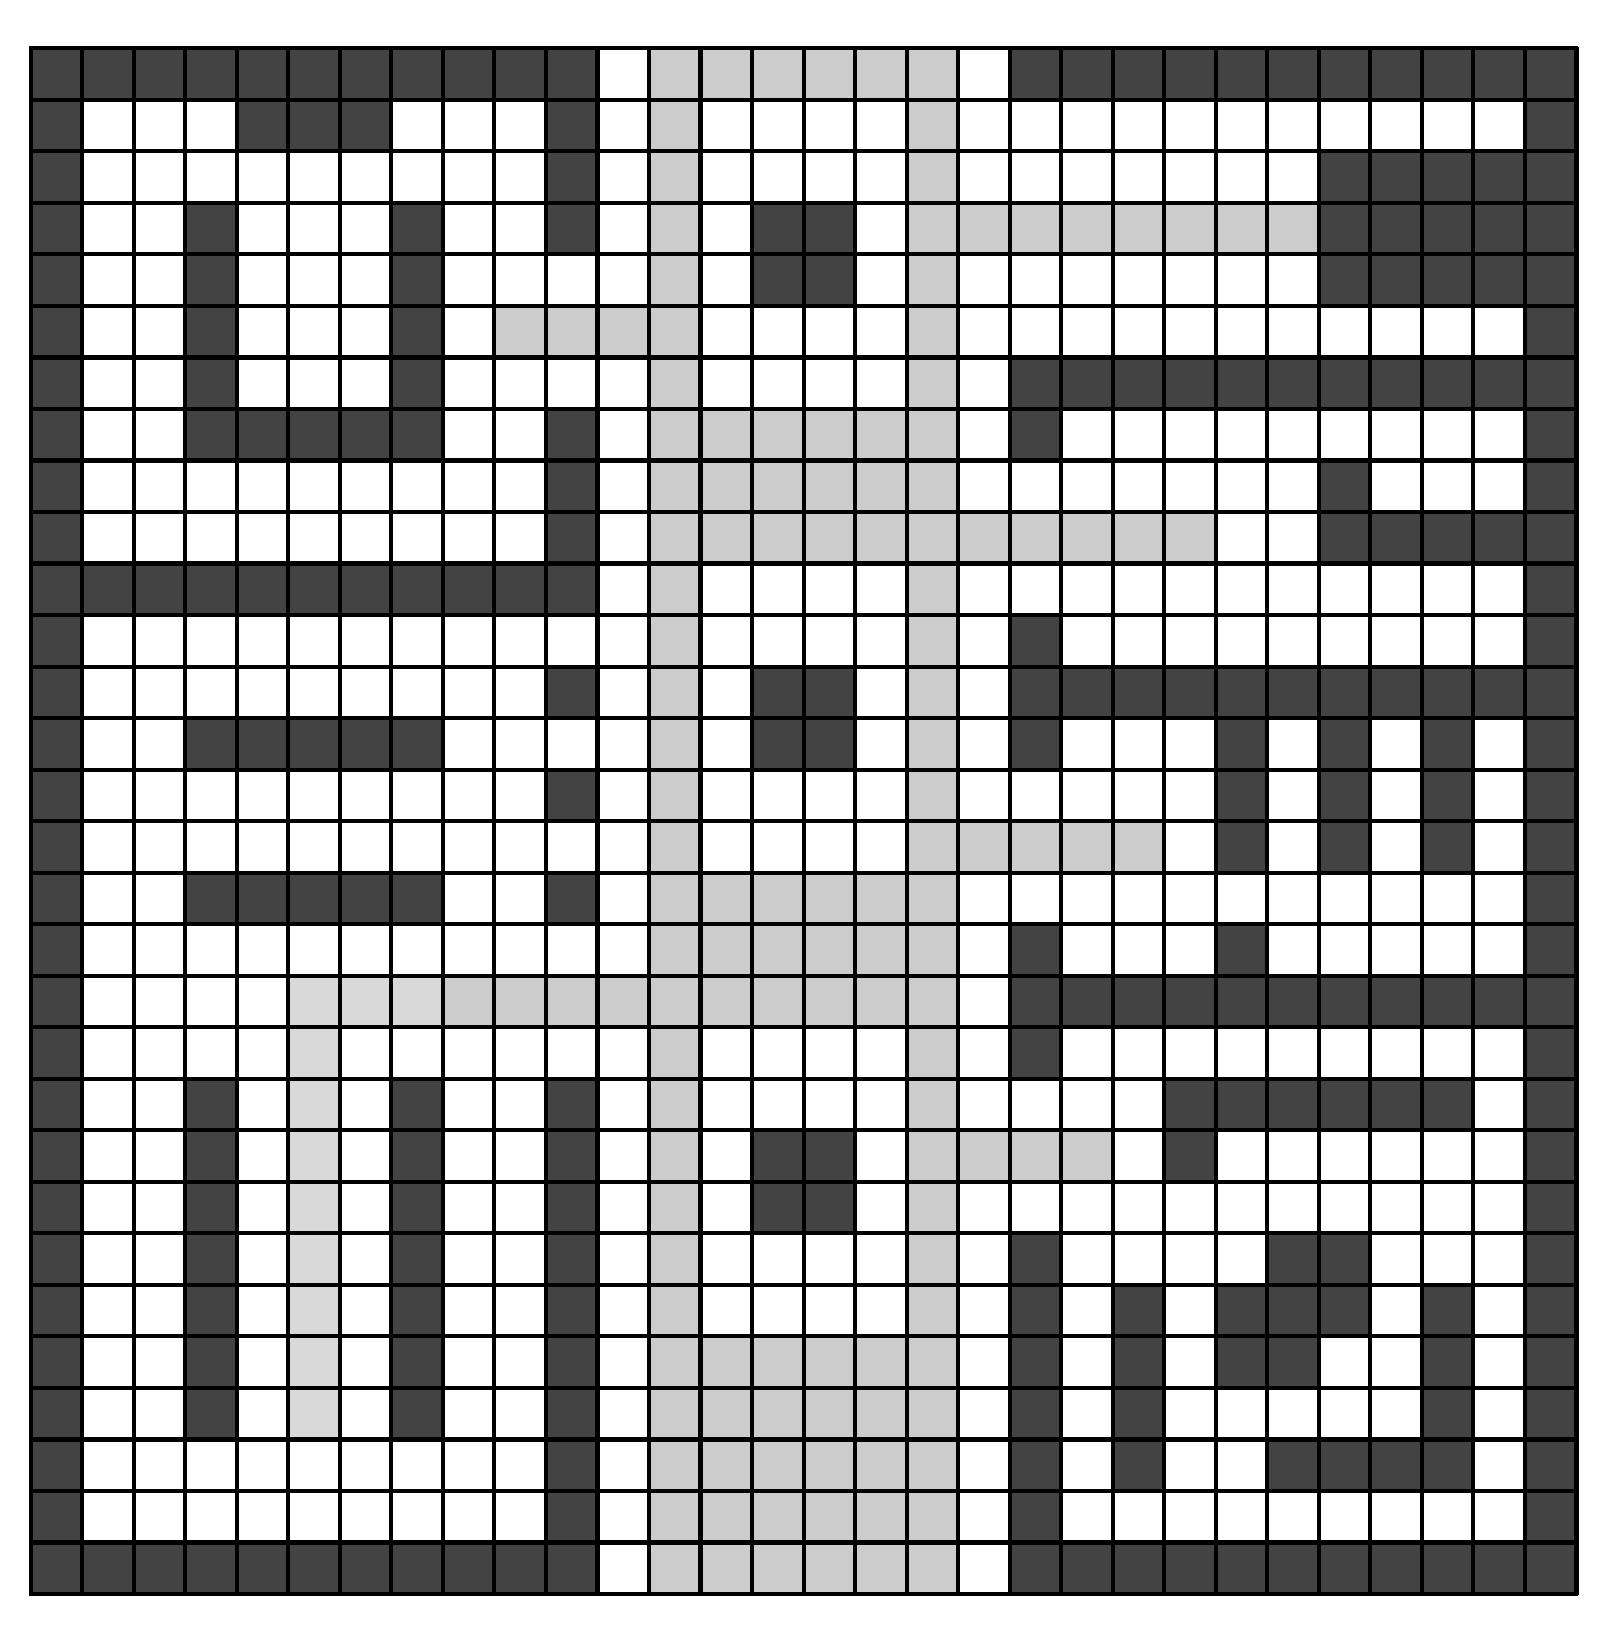
\includegraphics[scale=0.2]{./img/MallLayout.pdf}
            \caption{Przykładowy rozkład pomieszczeń małego centrum handlowego.}
            \label{fig:mall-layout}
        \end{figure}

        \begin{figure}[H]
            \centering
            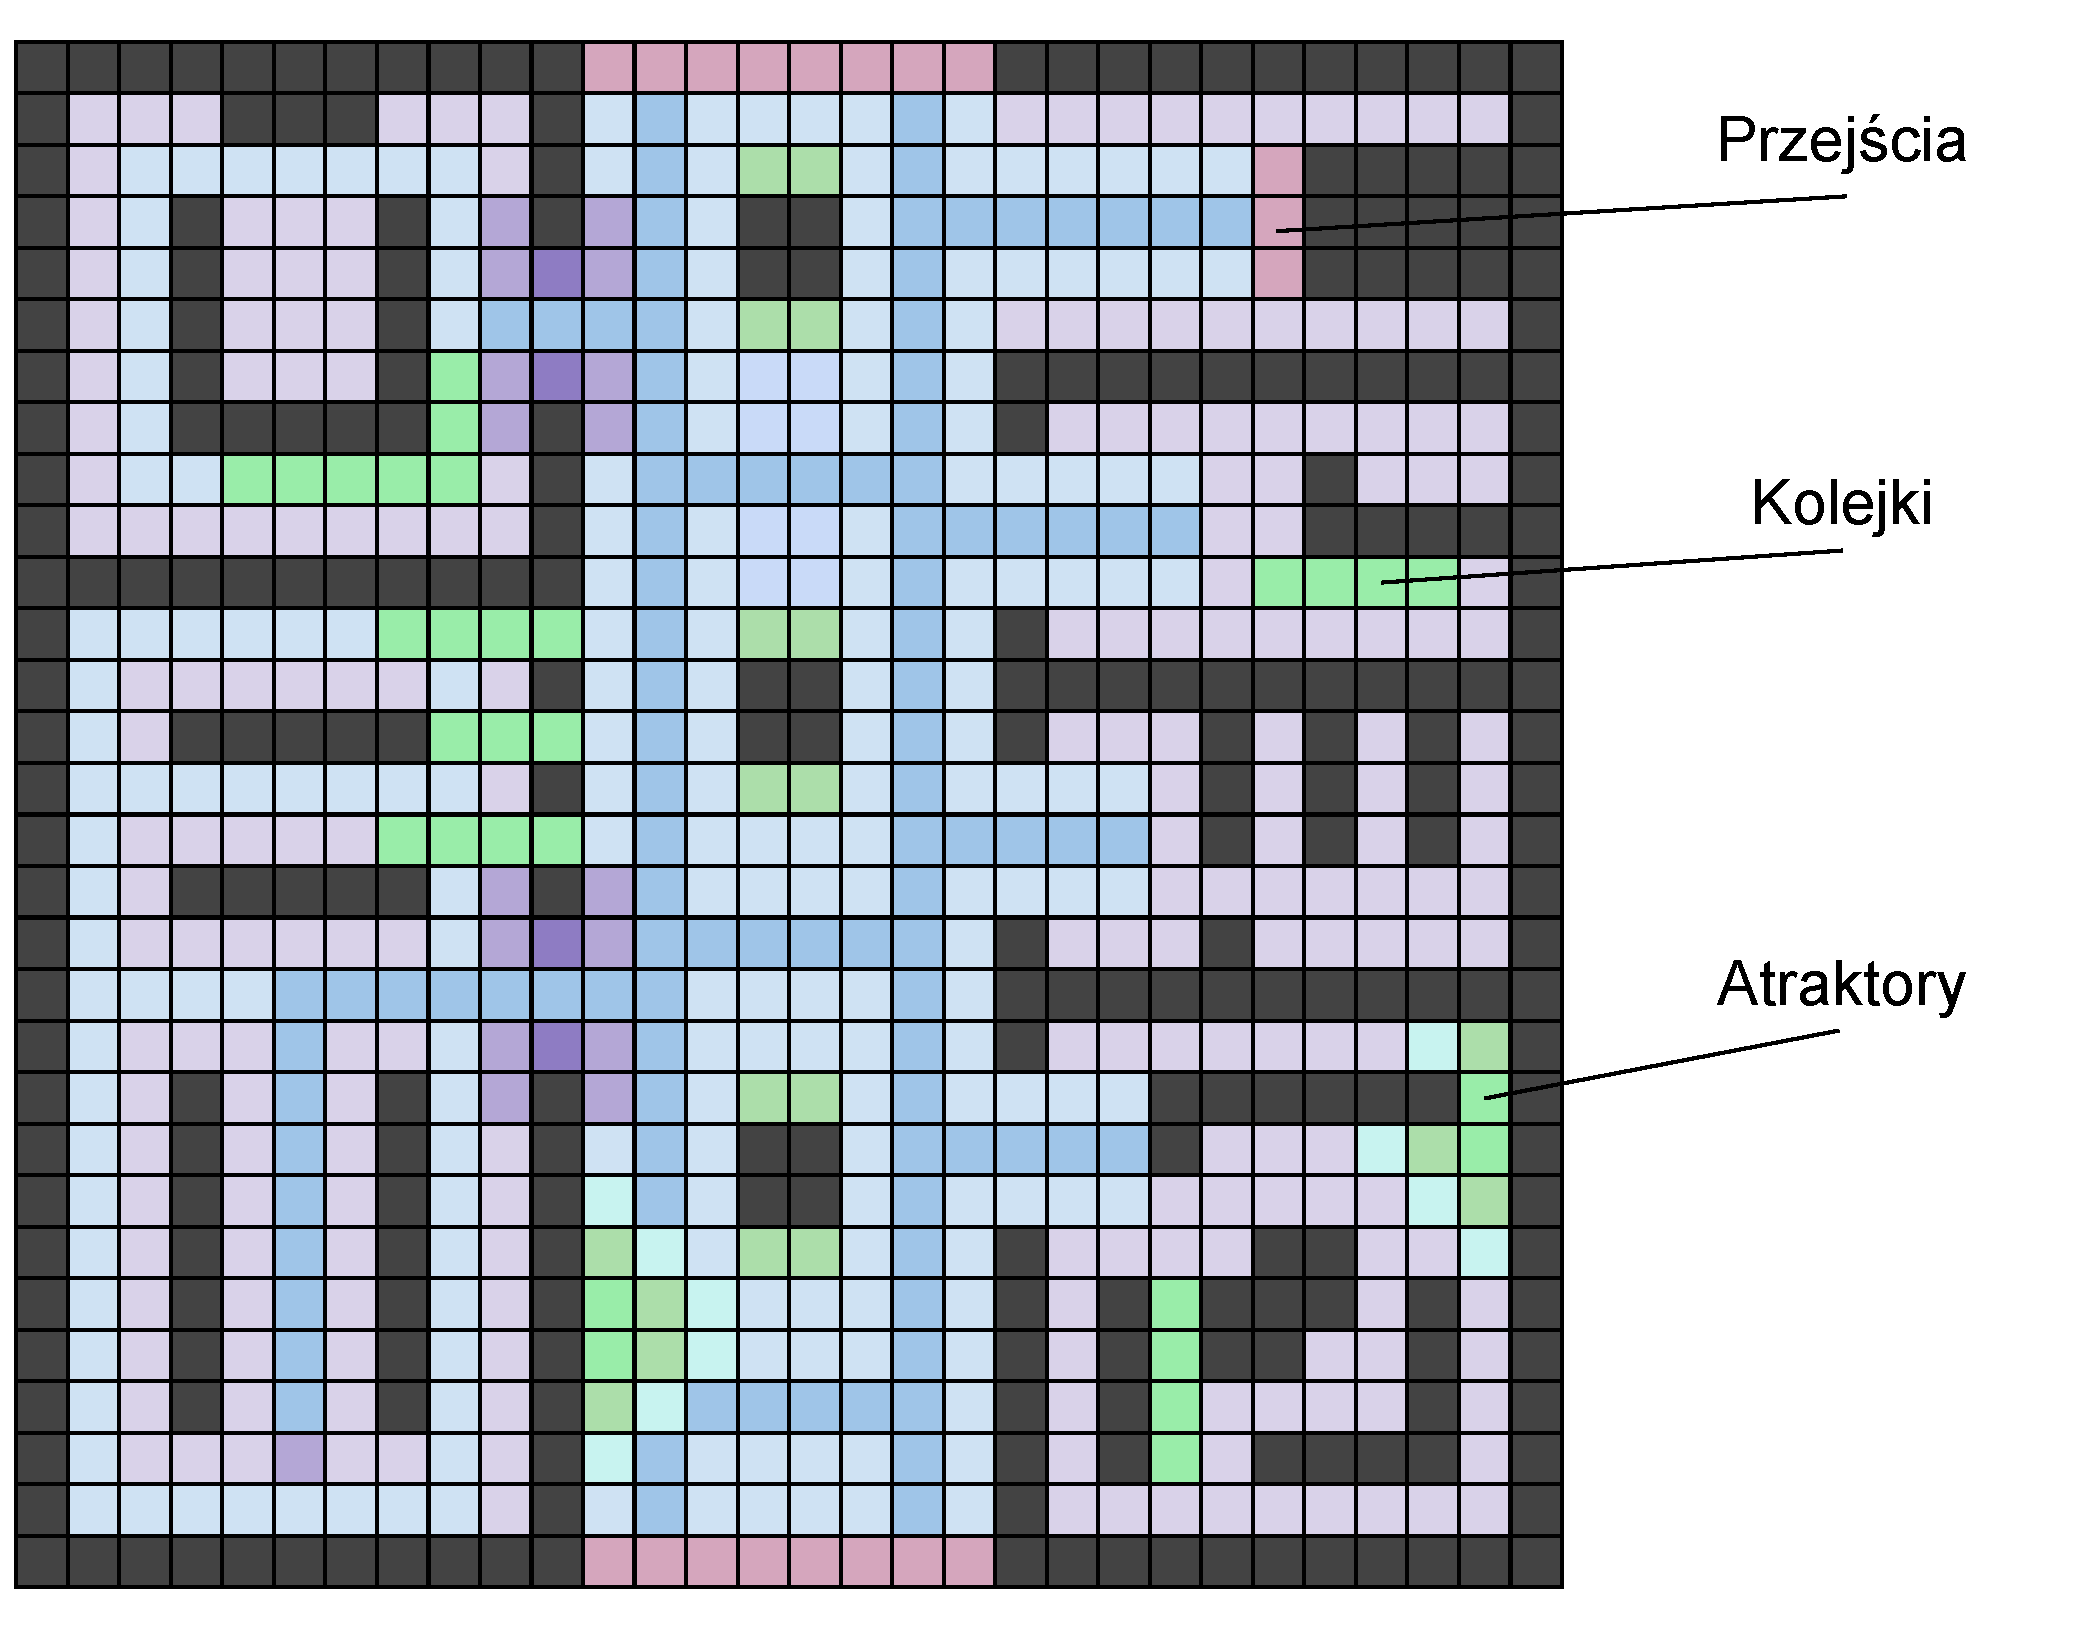
\includegraphics[scale=0.2]{./img/MallFeatures.pdf}
            \caption{Przykładowy rozkład stref specjalnych małego centrum handlowego.}
            \label{fig:mall-features}
        \end{figure}

        % TODO Opisać jak obsługiwane są wielopiętrowe centra handlowe.
        % TODO Opisać, jak kodowane są poszczególne strefy specjale.

        \subsection{Reprezentacja agentów}
        \label{sec:actor-impl}

        % TODO Opisać parametry agentów.

        \subsection{Wybór puntków docelowych}
        \label{sec:destination-choice}

        % TODO Opisać, jak wybierane są punkty docelowe.

        \subsection{Znajdowanie ścieżek}
        \label{sec:path-finding}

        % TODO Opisać algorytm A*.

        \subsection{Dewiacja ścieżek}
        \label{sec:path-deviation}

        % TODO Opisać wpływ różnych stref specjalnych na wygenerowane ścieżki.

        \subsection{Ruch agentów}
        \label{sec:movement-impl}

        % TODO Opisać konkretny algorytm poruszania się agentów (czy to CA-ped czy ped-4).

        \subsection{Preferencje odległościowe agentów}
        \label{sec:social-dist}

        % TODO Opisać implementację Social Distances w tym projekcie.

\newpage
    \section{Symulacja i analiza wyników}
    \label{sec:sim}

    % TODO Stworzyć i opisać przykładowy problem (albo dwa), takie jak mały sklep, czy duże centrum.
    % TODO Zasymulawać przykładowy problem i zebrać dane.

        \subsection{Kalibracja i walidacja parametrów symulacji}
        \label{sec:p}

        % TODO Opisać metody kalibracji i walidacji parametrów symulacji.

        \subsection{Uzyskane wyniki ilościowe i jakościowe}
        \label{sec:results}

        % TODO Opisać otrzymane wyniki, przedstawić statystyki zachowań,
        % TODO czasów spędzonych w centrum handlowym itp.

        \subsection{Wyniki symulacji a rzeczywistość}
        \label{sec:sim-vs-reality}

        % TODO Napisać dokładne porównanie z rzeczywistymi danymi.

\newpage
    \begin{thebibliography}{9}
        \label{sec:refs}

        \bibitem[Wąs, Gudowski, Matuszyk]{refs:social-distances-1} - Social Distances Model of Pedestrian Dynamics
        \bibitem[Karakayali]{refs:social-distances-2} - Social Distance and affective orientation
        \bibitem[Bogardus]{refs:group-relations} - Measurement of personal-group relations

        \bibitem[Blue, Adler]{refs:4-way-movement} - Modelling Four Directional Pedestriam Movements
        \bibitem[Blue, Adler]{refs:cellural-movement} - Cellural automata microsimulation for modeling bi-directional pedestrian walkways
        \bibitem[Bitgood, Dukes]{refs:movement-economy} - Economy of Movement and Pedestrian Choice Point Behavior in Shopping Malls
        \bibitem[Borgers, Timmermans]{refs:route-choice-1} - A Model of Pedestrian Route Choice and Demand for Retail Facilities within Inner-City Shopping Areas
        \bibitem[Borgers, Timmermans]{refs:route-choice-2} - City centre entry points, store location, patterns and pedestrian route choice behaviour: a microlevel simulation model
        \bibitem[Borgers, Timmermans]{refs:pedestrian-behaviour-1} - Modelling pedestrian behaviour in downtown shopping areas
        \bibitem[Kitazawa, Batty]{refs:pedestrian-behaviour-2} - Pedestrian Behaviour Modelling
        \bibitem[Zacharias]{refs:real-data-1} - Shopping behavior at Alexis-Nihion Plaza in Montreal
        \bibitem[Rauh, Schenk, Schrődl]{refs:real-data-2} - The Simulated consumer - an agent-based approach to shopping behaviour
    \end{thebibliography}
\end{document}
